
\documentclass[a4paper]{article}
\usepackage{amsmath}

\usepackage{tikz}
\usetikzlibrary{bayesnet}


\begin{document}
\pagestyle{empty}
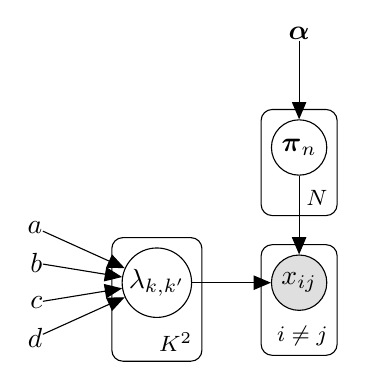
\begin{tikzpicture}
    \node[obs]                  (xij) {$x_{ij}$};
    \node[latent, above=of xij] (pi) {$\boldsymbol{\pi}_n$};
    \node[const, above=of pi] (alpha) {$\boldsymbol{\alpha}$};
    \node[latent, left=of xij] (lambda) {$\lambda_{k,k'}$};
    \node[const, left=of lambda, yshift=0.7cm] (a) {$a$};
    \node[const, left=of lambda, yshift=0.25cm] (b) {$b$};
    \node[const, left=of lambda, yshift=-0.25cm] (c) {$c$};
    \node[const, left=of lambda, yshift=-0.7cm] (d) {$d$};

    \edge{alpha}{pi};
    \edge{pi}{xij};
    \edge{lambda}{xij};
    \edge{a,b,c,d}{lambda};

    \plate{}{(xij)}{$i\neq j$};
    \plate{}{(pi)}{$N$};
    \plate{}{(lambda)}{$K^2$}
\end{tikzpicture}
\end{document}

